% Prepinace pre figure:
% h=approximately here
% t=top of page
% b=bottom of page
% p=on special page
% H=precisely here
\newcommand{\InsertCode}[2]{\begin{figure}[#1]\input{#2}\end{figure}}

\newcommand{\Code}[1]{\texttt{#1}}

\chapter{Popular Data Processing Frameworks for Java \label{chapter:frameworks}}

In this chapter, we show basic features of chosen frameworks
that are used for manipulating data.
We focus on the basic features relevant for the data lineage
and ignore most of their advanced features.

We show data lineage basic examples of how data can be loaded or stored by Java application
and how sources and sinks are identified, as this is the main topic of our work.

All frameworks that are using database, would work with the example
of loading objects of the class \Code{DatabaseValue} in the Listing \ref{code:model}
from database structured as in \ref{code:db}.

\InsertCode{h}{code/model}

TODO RE model databaze:
\begin{lstlisting}[caption={Example of database}, label={code:db}]
TABLE T
ID  | VALUE
1   | A
2   | B
... | ...
\end{lstlisting}







\section{JDBC API \label{frameworks:jdbc}}

For accessing database in Java applications, there exists the standard
Java Database Connectivity (JDBC) API.
The API is described in more detail in \citet{JDBC_OVERVIEW}
and here we show just the features that are relevant for this work.

Database vendors usually provide JDBC API implementation. This API is generic, so
there should be no difference for connecting to different database types.

The main component of the API is the \Code{java.sql} \citep{java.sql} package.
We present main interfaces controlling database calls:
\begin{itemize}
  \item \Code{Connection}
  \item \Code{Statement}, \Code{PreparedStatement}, \Code{CallableStatement}
  \item \Code{ResultSet}
\end{itemize}

\Code{Connection} object should hold database connection and through this connection
database queries can be executed using any of \Code{Statement} calls.
When data are returned to application from statement, it is done through \Code{ResultSet}.

Getting connection to database is through \Code{DriverManager}, or since JDBC 2.0
it can be done using \Code{DataSource} and it is now the preferred way of connecting to database.
Listing \ref{code:datasource} shows how \Code{DataSource} can be created for Oracle database
that is listening on url \Code{jdbc:oracle:thin:@//192.168.0.16:1521/orcl}
and \Code{User} user and \Code{Password} password is used when connecting to it.

The \Code{createDataSource()} calls would be also used in next database examples.

\InsertCode{h}{code/datasource}

Code in Listing \ref{code:jdbc} shows how loading data from \Code{DataSource}
(as in \ref{code:datasource}) can be done using JDBC API.
On line \ref{code:jdbc:connection}, connection to database is created.
Then on lines \ref{code:jdbc:prepareStatement:begin}--\ref{code:jdbc:prepareStatement:end}
database query is created to select just rows matching \Code{id} argument.
The query is then executed on line \ref{code:jdbc:executeQuery} and then
result is mapped from \Code{ResultSet} to our \Code{DatabaseValue} model and then it is returned on line \ref{code:jdbc:return}.

\InsertCode{h}{code/jdbc}




\section{Spring JDBC Framework \label{frameworks:jdbcTemplate}}
\citet{SpringJDBC} is extension above JDBC API that tries to help developers to code only
parts with application logic and it removes much of the boilerplate code.
It is illustrated by next list from \citet{SpringJDBC}, from which only
italicized items need to be coded by user, and all low level details
are handled by framework:
\begin{itemize}
  \item Define connection parameters
  \item Open the connection
  \item \textit{Specify the statement}
  \item Prepare and execute the statement
  \item Set up the loop to iterate through the results (if any)
  \item \textit{Do the work for each iteration}
  \item Process any exception
  \item Handle transactions
  \item Close the connection   
\end{itemize}

Before Java 7, coding in standard JDBC tend to be errorneus because of forgetting to close
database resources (user needs to close resources in finally block as try-with-resources did not exist yet)
and the boilerplate code does not help in readability of code.

Listing \ref{code:jdbcTemplate} illustrate loading single row from database.
Framework uses \Code{RowMapper} objects, that define transformation of
each row in query result to user defined object.
On the line \ref{code:jdbcTemplate:mapper}, we define \Code{Mapper} class
for transforming rows to resulting \Code{DatabaseValue}.
We can notice, that transformation done by \Code{Mapper} is the same as it was in JDBC example
in Listing \ref{code:jdbc} on lines \ref{code:jdbc:mapping:begin}--\ref{code:jdbc:mapping:end}.
Framework handles all boilerplate code around and result is returned
after processing single line \ref{code:jdbcTemplate:return}.


\InsertCode{h}{code/jdbcTemplate}





\section{MyBatis Framework \label{frameworks:myBatis}}

\citet{MyBatis} is one of Object-Relational Mapping (ORM) frameworks.
It internally uses JDBC API to communicate with the database, but in almost all cases,
there is no need to work with the low level JDBC.

Unlike other ORM frameworks, it does not map Java objects to database tables, but Java methods
to SQL statements. Framework uses concept of \Code{Mapper} interfaces (but differently as Spring JDBC Framework).
Developer define \Code{Mapper} interface with some methods, that executes SQL queries,
and all communication with database is always happening through these methods.

For each method SQL query is defined and when some output is expected,
mapping of rows to Java objects should be provided.
Name \Code{Mapper} is derived from the feature of mapping database query result
to Java objects.
Definition of queries and mappings could be done by
external XML files or by annotations in these interfaces.

In section \ref{frameworks:myBatis:mapper} we show examples of \Code{Mapper} interface,
in section \ref{frameworks:myBatis:configuration} we show how database configuration
can be created and in section \ref{frameworks:myBatis:run} we finally show how to
use these parts to load data from database.




\subsection{Mapper definition \label{frameworks:myBatis:mapper}}

In this section, we show examples of \Code{Mapper} interface definition
for MyBatis Framework done by XML and also by annotations.

When using \Code{Mapper} interface, framework internally create implementation
of it and by calling its methods, the same logic is done as
in previous JDBC example, when connection to database is open
and \Code{PreparedStatement} is created with defined query and provided arguments,
and after execution is done, resulting object values are mapped from \Code{ResultSet}.

Listing \ref{code:mybatis:interface:annotations} uses annotations to store definitions
of both query and mapping for method \Code{getForId} defined on line
\ref{code:mybatis:interface:annotations:method}. Line \ref{code:mybatis:interface:annotations:query}
contains query definition using the \Code{@Select} annotation and lines
\ref{code:mybatis:interface:annotations:result:begin}--\ref{code:mybatis:interface:annotations:result:end}
contains mapping of result columns to \Code{DatabaseValue} attributes
using the \Code{@Results} and \Code{@Result} annotations.

\InsertCode{h}{code/mybatis-interface-annotations}

Listing \ref{code:mybatis:interface:xml} shows the same functionality but using XML.
First, method \Code{getForId} is defined in interface and the rest,
query and mapping, is stored in XML mapper file.
Query is located on line \ref{code:mybatis:mapper:xml:query} in \Code{<select>} tag.
Tag contains a reference to the correct \Code{resultMap} mapping on lines
\ref{code:mybatis:mapper:xml:mapping:begin}--\ref{code:mybatis:mapper:xml:mapping:end},
which contains mapping of result columns to \Code{DatabaseValue} object attributes.

\InsertCode{h}{code/mybatis-interface-xml}



\subsection{Configuration \label{frameworks:myBatis:configuration}}

The main MyBatis component responsible for creating database connections
is \Code{SqlSessionFactory}. It needs to be configured to successfully connect
to database. Configuration can be done in Java or using external XML configuration file.

In Listing \ref{code:mybatis:sessionFactory:java} we show, how configuration can be
done in Java. On line \ref{code:mybatis:sessionFactory:java:dataSource} we use \Code{DataSource},
that we previously define in Listing \ref{code:datasource}.
\Code{JdbcTransactionFactory} was used to handle database transactions.
On line \ref{code:mybatis:sessionFactory:java:addMapper} \Code{Mapper} interface is registered
to be known by MyBatis and finally \Code{SqlSessionFactory} is created.

\InsertCode{h}{code/mybatis-sessionFactory-java}

In Listing \ref{code:mybatis:sessionFactory:xml} we show, how configuration can be
done using external XML file. \Code{SqlSessionFactory} is created
on line \ref{code:mybatis:sessionFactory:xml:file}. Configuration file
configures \Code{DataSource} on lines
\ref{code:mybatis:configuration:xml:dataSource:begin}--\ref{code:mybatis:configuration:xml:dataSource:end}
and \Code{Mapper} interface is registered on line \ref{code:mybatis:configuration:xml:mapper}.

\InsertCode{H}{code/mybatis-sessionFactory-xml}




\subsection{Loading Data from Database \label{frameworks:myBatis:run}}

Since we know how to configure database connections and how to define mappers,
we are ready to show how data can be loaded from database.
Listing \ref{code:mybatis} show all pieces together. First, on line
\ref{code:mybatis:sqlSessionFactory} we create previously configured
\Code{SqlSessionFactory} from which we open \Code{SqlSession} to
access database. On line \ref{code:mybatis:getMapper} implementation
of \Code{Mapper} interface is retrieved and on line \ref{code:mybatis:return}
database query is executed and its result is returned. 

\InsertCode{H}{code/mybatis}



\section{Kafka \label{frameworks:kafka}}

Apache \citet{Kafka} is a distributed streaming platform.
It means that application can publish or subscribe records and
process them, as they occur.

Kafka can run as a cluster on one or more servers.
Each cluster stores stream of records in categories that are called \textit{topics}.
Topics can be viewed as database tables. Producers write to a topic's table
and consumers read new data from that table.
When application wants to publish some records (producer) in the topic,
it sends them to server from which data are forwarded to all its subscribers (consumers).

Topics can be also partitioned, so distributed computations can be made
on them - each partition can be handled by different server (or producer or consumer).
Partitions are ordered, immutable sequences of records that are continually appended to.

Structure of data in records can be arbitrary. Application just need to handle
correct transformation of used Java object to (or from) byte array using
\Code{Serializer} (or \Code{Deserializer}) objects.
However, this feature is not very important considering data lineage problem\footnote{
  We cannot distinguish values that belong to same attribute, as it was in case
  of databases, where rows were divided into columns and we could make
  lineage on attribute/column level.
}.

The Kafka cluster durably persists all published records (whether or not they have been consumed)
using a configurable retention period. For that period, any consumer can access
to any published record.

Figure \ref{frameworks:kafka:api} and next list from \citet{Kafka}
illustrates usage of four Kafka core client APIs:
\begin{itemize}
  \item The \textbf{Producer API} (see section \ref{frameworks:kafka:producer}) allows an application to publish
    a stream of records to Kafka topics
  \item The \textbf{Consumer API} (see section \ref{frameworks:kafka:consumer}) allows an application to subscribe
    to topics and process the stream of records produced to them
  \item The \textbf{Streams API} (see section \ref{frameworks:kafka:streams}) allows an application to act as a stream processor,
    consuming an input stream from topics and producing an output stream to output topics,
    effectively transforming the input streams to output streams
  \item The \textbf{Connector API} (see section \ref{frameworks:kafka:connector}) allows building and running reusable producers or consumers
    that connect Kafka topics to existing applications or data systems.
    For example, a connector to a relational database might capture every change to a table. 
\end{itemize}

\begin{figure}[h]
  \center
  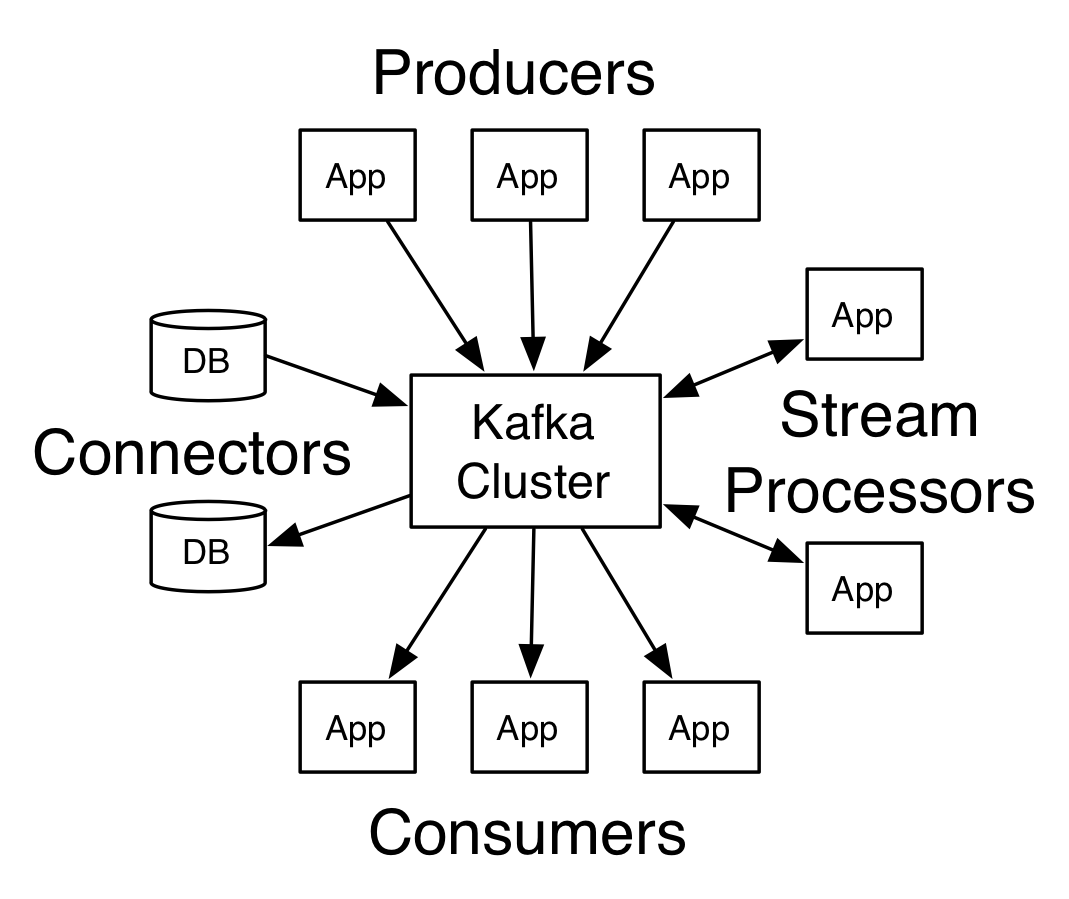
\includegraphics[width=100mm]{img/kafka-apis.png}
  \caption{Applications using differend kinds of Kafka APIs}
  \label{frameworks:kafka:api}
\end{figure}




\subsection{Producer API \label{frameworks:kafka:producer}}

Using Kafka Producer API, application can create new records and send them to topic of Kafka server.
It illustrates example in Listing \ref{code:kafka:producer}.
We first configure \Code{KafkaProducer} and then we just send records to topic \Code{Topic}
to Kafka server by calling \Code{send} method. We do not need to deal with the \Code{Serializer}s,
as they are provided for some basic Java classes (like \Code{String}) by framework itself.

\InsertCode{h}{code/kafka-producer}



\subsection{Consumer API \label{frameworks:kafka:consumer}}

Using Kafka Consumer API, application can handle new records that are arriving from server.
Receiving such data shows Listing \ref{code:kafka:producer}.
We also configure \Code{KafkaConsumer} as in previous section.
On line \ref{code:kafka:consumer:subscribe} we call \Code{subscribe}
to register consumer to receive records in topic \Code{Topic}.
On line \ref{code:kafka:consumer:poll} server is queried for new data.
We use 1 second as maximal time limit, for which Kafka waits for new records to
arrive and then such records are returned and we can handle them.

\InsertCode{h}{code/kafka-consumer}



\subsection{Stream API \label{frameworks:kafka:streams}}

A Kafka Stream represents an unbounded, continuously updating data set.
It is an ordered, replayable, and fault-tolerant sequence of immutable data records.
Application defines its computational logic through processor topologies,
where processor topology is a graph of stream processors (nodes) that are
connected by streams (edges).

Stream processor is a node in the processor topology, that represents
a processing step to transform data in streams by receiving one
input record at a time from its upstream processors in topology,
applying its operation on it and then produce one or more
output records to its downstream processors.

In topology, there are two special processors:

\TODO{Zacinat velkym The? Pripadne to davat ako vety? .. rovnako aj v bodoch v kafka api}
\begin{itemize}
  \item The \textbf{Source Processor} is a stream processor
    that does not have any upstream processors. It produces an input stream
    to its topology from one or multiple Kafka topics by consuming records
    from these topics and forwarding them to its down-stream processors
  \item The \textbf{Sink Processor} is a stream processor
    that does not have down-stream processors. It sends any received records
    from its up-stream processors to a specified Kafka topic.
\end{itemize}

The way, how topology can be defined is using the Kafka Streams DSL (Domain Specific Language).
It provides the most common data transformation operations, such as
\Code{map}, \Code{filter}, \Code{join} and \Code{aggregations}.
There exists also the low level Processor API, that allows developers define
and connect custom processors and also interact with state stores.




\subsection{Connector API \label{frameworks:kafka:connector}}

A Kafka Connector is a tool for scalably and reliably streaming data between Kafka
and other systems. It makes it simple to quickly define connectors that move
large collections of data into and out of Kafka.
Kafka Connector can ingest entire databases or collect metrics from all
application servers into Kafka topics, making the data available
for stream processing with low latency.




\section{Requirements for Data Lineage Library \label{frameworks:requirements}}

In previous sections we demonstrated usage of different Java frameworks
that are usually used in Java applications to manipulate data.
We ignored their advanced features and showed some examples of reading
and writing data.

We described three types of data processing frameworks:
\begin{itemize}
  \item \textbf{Spring JDBC Framework}, that just simplify the standard JDBC API,
  \item \textbf{MyBatis Framework}, which is the ORM framework,
  \item \textbf{Kafka Framework}, which is the distributed streaming platform.
\end{itemize}

In the rest of this section, we point out requirements of library, that
would be needed to successfully create data lineage of such applications.

The library should \textbf{analyse} whole \textbf{Java application} with all
its dependencies to know what calls are executed from some
entrypoint method (like \Code{main} method in Java, but in
our analysis it can be arbitrary method).

It is also important to \textbf{know concrete values} of some elementary Java
objects, such as \Code{String}s or number types, to know
what database is application connecting to, what SQL statement
it executes etc.

The library should be able to work with \textbf{external files}
as many frameworks store configuration outside the code.

The \textbf{callback}s are also important to handle by library
as many frameworks use them to asynchronously notify application about
some task result (failed, done), or even to simplify the usage of other API.

The last, but not least library requirement is to be able to easily
\textbf{extend to support new frameworks}. It is very important,
as new and new frameworks are developed and library should be ready
to add support for creating their data lineage.




